\documentclass[12pt,twoside]{article}
\usepackage{light}
\usepackage{subfigure}
\usepackage{graphicx}
%\hidesolutions
\showsolutions


\begin{document}

\problemset{5}{September 30, 2014}{Monday, October 6} 
\noindent \textbf{Reading Assignment:}   Sections 5.4.1--5.4.2, 5.5--5.7, 6.1--6.3
\\








% P1
\begin{problem}{16} 

  In the cycle $C_{2n}$ of length $2n$, we'll call two vertices
  \emph{opposite} if they are on opposite sides of the cycle, that is
  that are distance $n$ apart in $C_n$.  Let $G$ be the graph formed
  from $C_{2n}$ by adding an edge, which we'll call a \emph{crossing
    edge}, between each pair of opposite vertices.  So $G$ has $n$
  crossing edges.

\bparts

\ppart{6} Give a simple description of the shortest path between any two
vertices of $G$.

\emph{Hint: Argue that a shortest path between two vertices in $G$ uses at
most one crossing edge.}

\solution{
  Suppose a path, $Q$, in $G$ begins with a crossing edge, then
  follows a path, $P$, in $C_{2n}$ and ends with another crossing
  edge.  Replacing every vertex in $P$ by its opposite, you get a walk
  in $C_{2n}$ between the endpoints of $Q$, but the new walk is two
  edges shorter than $Q$.  This implies that a \emph{shortest} path in
  $G$ uses at most one crossing edge.

  A path $Q$ that uses exactly one crossing edge will have the
  following form: it follows a path $P_1$ in $C_{2n}$, then a crossing edge,
  and then another path $P_2$ in $C_{2n}$. We could describe another
  path by first following a crossing edge, then all of the
  opposite edges of path $P_1$, and then $P_2$; this path has the same
  length.

  So it suffices to consider the following two candidates for the shortest
  path from $v$ and $w$.
  The first candidate follows a crossing edge to the opposite $v'$ of $v$,
  and then navigates around the cycle $C_{2n}$ to the target vertex $w$. The
  second candidate uses no crossing edges, and simply navigates around
  $C_{2n}$. The first of these has length $1 + c_{v'w}$, and the second
  of these has length $c_{vw}$; so to find a shortest path from $v$ to
  $w$, we compare these two quantities and choose either the first or
  second candidate to yield the smaller length.

  We can even write $c_{v'w} = n - c_{vw}$; then we choose the first candidate
  when $1 + n - c_{vw} \leq c_{vw}$, i.e.\ when $c_{vw} \geq \frac{n+1}{2}$,
  and otherwise choose the second candidate.
}

\ppart{3} What is the \emph{diameter} of $G$, that is, the largest
distance between two vertices?

\solution{
    If $n=2k$ the diameter is $k$.  If $n = 2k + 1$ the diameter
  is also $k$.  (For $d \in [1,n)$ find the maximum value of
    $\min(d,1+n-d)$.)
}

\ppart{3} We say that a graph is \emph{$k$-edge connected} if removing
  $(k-1)$ edges can not disconnect the graph. Prove that the graph above is
  not 4-edge connected.

\solution{
    Every vertex of the graph has degree $3$.  Removing all $3$
  edges incident to a vertex disconnects the graph.  (If it was
  $4$ connected, no matter what $3$ edges we remove, the graph would
  have to remain connected.)
  }

\ppart{4} Prove that the graph is 3-edge connected.

\solution{
    Let $G'$ be the graph that remains after removing two edges.
  Removing any two edges that were orginally part of $C_{2n}$ splits
  $C_{2n}$ into two connected components, each of them paths.  Call
  them $P$ and $P'$.  Since the length of the paths and the two
  removed edges sum to $2n$, one path must have length at most $n-1$.
  Call this one $P$.  Pick a vertex $v$ within $P$.  $v$ is distance
  $n$ to some other vertex, $w$, in $C_{2n}$.  So $w$ must be in the
  other path $P'$.  The paths $P$, $P'$, and the edge $(v,w)$
  form a spanning tree in $G'$ which then must be connected.

  Removing at most one edge from $C_{2n}$ leaves $C_{2n}$ connected,
  hence $G'$ remains connected too.
  }

\eparts
\end{problem}








% P2
\begin{problem}{14} 

    Bruce and Sam have been told that there is a bomb on a street intersection, lying in a region of Manhattan for which the street map forms a $19 \times 7$ undirected grid. (Vertices are street intersections, and edges are single blocks of a street). The bomb is on one street intersection, and the code that they need to defuse the bomb is on another street intersection.

    Starting from where the bomb is, Bruce and Sam need to check all $19 \cdot 7 = 133$ street intersections for the code. Once they are at an intersection, they don't need any additional time to verify whether the code is there. Once they find the code and return to the bomb, they can disarm it in $2$ minutes. Also, they can run one block (in any of the four directions) in exactly $1$ minute. They are given 135 minutes total to find the code and disarm the bomb, which means that they need to return to the bomb, code in hand, in 133 minutes.

    Sam realizes that they need to use a cool new 6.042 concept: a \emph{Hamiltonian cycle} is a path that visits each vertex in a graph exactly once and ends at its starting point (so it is a cycle). A graph is \emph{Hamiltonian} if it has an Hamiltonian cycle. Sam is very excited because he thinks he can show that this region of Manhattan is Hamiltonian. If it is, Bruce and Sam can save the day! Will they make it?

\bparts

\ppart{5} Show that they cannot do it -- that is, more generally, show that if both $N$ and $M$ are odd, then the $N \times M$ grid is \emph{not} Hamiltonian.
\emph{Hint: First show that any $N \times M$ 2-dimensional undirected grid is bipartite.}
\solution{
    Any $2$-dimensional undirected grid is bipartite. To show this fact, let us exhibit a coloring of such a grid with $2$ colors $\{0,1\}$: indexing the vertices of the grid by their $(x,y)$-coordinates, we color vertex $(i,j)$ with color $\mathrm{rem}(i+j,2)$. The resulting colored grid now has each vertex adjacent to only vertices in the other color. Since any connected graph that can be colored by two distinct colors is bipartite, any $N \times M$ $2$-dimensional undirected grid is bipartite.

    Suppose the $N \times M$ grid is Hamiltonian. Since $N$ and $M$ are both odd, there is an odd number of vertices in the grid. It follows that the Hamiltonian cycle in this grid is an odd cycle. However, since we have already shown that any $2$-dimensional undirected grid is bipartite, odd cycles are not possible. We have reached a contradiction; thus, our supposition that the grid was Hamiltonian is wrong, and we are done.
}


\ppart{9} Suppose we defined Midtown in the more standard way as extending from 40th Street to 59th Street and from 3rd Avenue to 9th Avenue (a $20 \times 7$ grid), and gave them another $7$ minutes.
\begin{enumerate}
    \item Show that if either $N$ is even and $M > 1$ or $M$ is even and $N > 1$, then the $N \times M$ grid is Hamiltonian.

        \solution{
            Suppose $N$ is even (WLOG). We can write a direct proof or an inductive proof.

            \emph{Direct constructive proof:} Assume the grid is laid out on the plane occupying the integer points between $(0,0)$ and $(N-1,M-1)$. We find the Hamiltonian path explicitly by specifying the $k$th vertex visited for each $k$ from $0$ to $NM$. Let $q = \lceil \frac{k}{M-1} \rceil$ and let $r = \mathrm{rem}(k,M-1)$.

            On step $k$:
            \begin{itemize}
                \item if $k \leq N(M-1)$ and $q$ is even, then visit vertex $(q,r+1)$;
                \item if $k \leq N(M-1)$ and $q$ is odd, then visit vertex $(q,M-1-r)$;
                \item if $k > N(M-1)$, then visit vertex $(0, N-(k-N(M-1)))$.
            \end{itemize}
            Checking that it is a Hamiltonian cycle is routine. Figure~\ref{2b-fig1} shows a picture of such a cycle. Thus, we conclude that the $N \times M$ grid is Hamiltonian.
            \begin{figure}
                \begin{center}
                    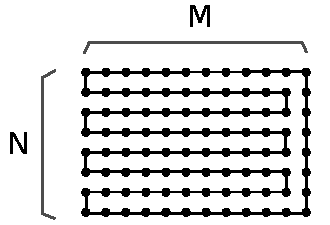
\includegraphics[scale=1.5]{ps5-figs/2b-fig1.pdf}
                \caption{Hamiltonian cycle described in solution for 2b.}
                \label{2b-fig1}
            \end{center}
            \end{figure}

            \emph{Inductive proof (also constructive):} We induct on even $N$ values. For the base case $N=2$, our cycle just has all the exterior edges of the grid. For the inductive step, we assume the existence of a Ham-cycle $H$ on an $N \times M$ grid, and construct a Ham-cycle on the $(N+2) \times M$ grid.

            Consider vertex $v = (N-1,0)$, lying at one `corner' of the original grid. By the definition of Ham-cycle, $H$ must include $v$, and thus $v$ is incident to $2$ distinct edges. There are only $2$ such edges possible on the grid, and in particular the edge $((N-1,0),\; (N-1,1))$ must be in $H$. We remove this edge and add the following edges:
            \begin{itemize}
                \item $((N-1,0),\;(N,0))$,
                \item $((N,0),\;(N+1,0))$,
                \item $((N,i),\;(N,i+1))$ for $1 \leq i < M$,
                \item $((N+1,i),\;(N+1,i+1))$ for $0 \leq i < M$,
                \item $((N,M-1),\;(N+1,M-1))$.
            \end{itemize}
            See Figure~\ref{2b-fig2} for an illustration. Thus we conclude that the $N \times M$ grid is Hamiltonian.
            \begin{figure}
                \begin{center}
                    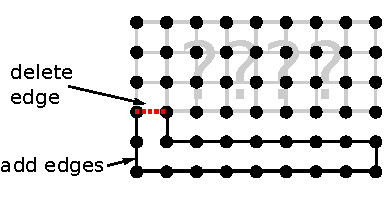
\includegraphics[scale=1.5]{ps5-figs/2b-fig2.pdf}
                \caption{Inductive construction of a Hamiltonian cycle.}
                \label{2b-fig2}
            \end{center}
            \end{figure}
        }

    \item Explain why your proof breaks down when $N$ and $M$ are odd.

        \solution{
            For the direct proof, the odd/even conditions on $q$ require $N$ to be even for the above sequence of vertices to actually form a cycle. For the inductive proof, the inductive step increases $N$ by $2$, and the only base case given is $N=2$.
        }

    \item Would they survive? Does the outcome depend on where the bomb is placed?

        \solution{
            Come on, Bruce and Sam would survive, of course! The number of steps taken around the Hamiltonian cycle doesn't depend on the starting vertex.
        }

\end{enumerate}

\eparts
\end{problem}










% P3
\begin{problem}{16}
    \bparts

    \ppart{8} Prove that a simple connected graph with $n$ nodes and $n-1$ edges is a tree.
    \solution{
        To show that a connected graph $G$ with $n$ nodes and $n-1$ edges is a tree, it is sufficient to show that it is acyclic. Assume to the contrary that there is a cycle in $G$; then we can remove an edge from this cycle while preserving connectivity. Then we have produced a connected subgraph $G'$ with $n$ vertices but only $n-2$ edges; this contradicts connectivity, and we conclude that the original graph must have been a tree.
    }

    \ppart{8} Prove by induction that any connected graph has a spanning tree.
    \solution{
        The proof is by induction on the number of edges. Let $P(k)$ be the predicate that if $G$ is connected with $k \geq n-1$ edges, then $G$ has a spanning tree.
        
        {\bf Base case}: $k = n-1$. Part (a) demonstrates that $G$ is a tree and thus a spanning tree of itself.

        {\bf Inductive step}: Assume $P(k)$. If $G$ is a connected graph with $k+1 > n-1$ edges, it must not be a tree, by part (a). It follows that $G$ must have a cycle. Removing an edge from that cycle creates a connected graph with $k$ edges, which has a spanning tree over the same nodes, by our inductive hypothesis. This spanning tree is also a spanning tree over $G$, thus $P(k+1)$ holds.

        By induction, a connected graph $G$ with $k$ edges has a spanning tree, for all $k \geq n-1$.
    }

    \eparts
\end{problem}







% P4
\begin{problem}{13}

    Let $G$ be a weighted undirected graph, and assume that $G$ is connected.
    
    \bparts

    \ppart{8} Suppose that $G$ contains a cycle $C$, and that we produce a subgraph $G'$ of $G$ by deleting a maximum-weight edge $e$ from $C$. Show that any minimum-weight spanning tree (MST) for $G'$ is an MST for $G$.

    \solution{
        Let $T'$ be a MST for $G'$, and suppose for a contradiction that $T'$ is not an MST for $G$. From lecture, we know that $G$ does have some MST $T$.

        If $G$ has an MST $T$ with $e \not\in T$, then $T$ is also a spanning tree for $G'$. As $T$ is minimal-weight for $G$, but $T'$ is not, we know that $T$ has lesser total weight than $T'$; so $T$ is a spanning tree for $G'$ with lesser weight than the MST $T'$, which is a contradiction. So the hypothesis of this paragraph must be false.

        So every MST $T$ of $G$ must contain $e$. Then $T$ must lack some other edge $e'$ from the cycle $C$, as $T$ is acyclic. If we remove $e$ from $T$ and add $e'$, we obtain another spanning tree $T''$, not containing $e$. But $e$ was chosen as a highest-weight edge from cycle $C$, so the weight of $e'$ is at most the weight of $e$, and the total weight of $T''$ is at most the total weight of $T$. As $T$ is an MST, and $T''$ has lesser-or-equal weight, we infer that $T''$ is an MST for $G$. But $T''$ does not contain $e$. This contradicts the first sentence of this paragraph.

        We are forced to conclude that the hypothesis at the very start of the solution was false. Every MST for $G'$ is an MST for $G$.
    }

    \ppart{5} Suppose that we iterate the process of part (a): while $G$ has a cycle $C$, find a highest-weight edge along $C$ and delete it. Prove that this procedure terminates in a minimum-weight spanning tree for $G$.

\solution{
    We proceed by induction on $m$, the number of edges in $G$. The base case is trivial: certainly the proposition is true for all connected weighted graphs with only a single edge, as these have no cycles and are always their own minimum-weight spanning trees.

    For the inductive step, suppose the proposition for all such graphs on $m-1$ edges. Given the graph $G$ with $m$ edges, we have two cases:
    
    \emph{Case 1}: $G$ has a cycle $C$. The procedure indicates to find a maximum-weight edge $e$ in $C$ and delete it, forming a graph $G'$. Notice that $G'$ has $m-1$ edges. Then the inductive hypothesis applies to $G'$: if we continue the procedure as indicated on $G'$, deleting edges from further cycles, we will obtain an MST for $G'$. By part (a), this is also an MST for $G$, completing the inductive step in this case..

    \emph{Case 2}: $G$ has no cycles. The procedure described in the problem will immediately terminate. As $G$ has no cycles, $G$ is already a tree; it is the only spanning tree for itself (since removing any edge will disconnect the graph), and therefore certainly has minimum weight. Thus the condition is satisfied, completing the inductive step. 

By induction, the proposition holds for all connected weighted undirected graphs $G$ of any size.
}

    \eparts

\end{problem}










% P5
\begin{problem}{10}
    
    Show that the congestion of the $N$-input butterfly is $\sqrt{N}$ if $N$ is an even power of $2$.

    \solution{
        First we will show that the congestion is at most $\sqrt{N}$.

        Let $v$ be an arbitrary vertex at some level $i$. Let $S_v$ be the set of inputs that can reach vertex $v$. Let $T_v$ be the set of outputs that are reachable from vertex $v$. Note that:
        \begin{itemize}
            \item For the butterfly network, there is a unique path from each input to each output, so the congestion is the maximum number of messages passing through a vertex for any matching of inputs to outputs.
            \item If $v$ is a vertex at level $i$ of the butterfly network, there is a path from exactly $2^i$ input vertices to $v$ and a path from $v$ to exactly $2^{n-i}$ output vertices.
        \end{itemize}

        We thus have $|S_v| = 2^i$ and $|T_v| = 2^{n-i}$. The number of inputs in $S_v$ that are matched with outputs in $T_v$ is at most $\min \{ 2^i, 2^{n-i} \}.$ To obtain an upper-bound on the congestion of the network, we need to find the maximum value of $\min \{ 2^i, 2^{n-i} \}$, where the maximum is taken over all $i$. The maximum value is achieved when $2^i$ and $2^{n-i}$ are as equal as possible. Since $n$ is even, these two quantities are equal when $i = \frac{n}{2}$, hence the maximum congestion is $2^{n/2} = N^{1/n} = \sqrt{N}$.

        So far, we have concluded that the congestion of $\sqrt{N}$ can only be achieved at a node at level $\frac{n}{2}$. Now consider the node at that level whose binary representation is all $0$s. Any packet from the input in the form $z\underbrace{0\ldots000}_{n/2\text{ bits}}$ with destination $\underbrace{000\ldots0}_{n/2\text{ bits}} z'$, where $z$ and $z'$ are any $\frac{n}{2}$-bit numbers, must pass through this node. In the worst case, all packets from input in the form $z\underbrace{0\ldots000}_{n/2\text{ bits}}$ will have destination in the form $\underbrace{000\ldots0}_{n/2\text{ bits}} z'$. But there are $2^{n/2} = \sqrt{N}$ such possible packets, giving the node load $\sqrt{N}$. Therefore, we can conclude that the congestion of $B_n$ is exactly $\sqrt{N}$ when $n$ is even.
    }

\end{problem}









% P6
\begin{problem}{20}

    In a \emph{perfect shuffle}, a deck of $N$ cards is cut exactly in half and then perfectly interlaced. Thus, for $N$ cards, we would obtain the resulting cards in the following order:
    $$ 1,\; \left(\frac{N}{2} + 1\right),\; 2,\; \left(\frac{N}{2} + 2\right),\; \ldots,\; \left(\frac{N}{2} - 1\right),\; \left(N - 1\right),\; \frac{N}{2},\; N. $$

    \bparts

    \ppart{10} Show that $m$ perfect shuffles will return a deck of $N$ cards to its original order provided that $2^m = 1 \pmod{(N-1)}$.

    \solution{
        Let $N \times m$ switches $P_0^1,\; P_1^1,\; \ldots,\; P_{N-1}^m$ be available, where $N = 2^m$ for some positive integer $m$. In this network of $N \times m$ switches, there is a one-way link connecting $P_i$ to $P_j$, where $j = 2i$ for $0 \leq i \leq \frac{N}{2} - 1$ and $j = 2i + 1 - N$ for $\frac{N}{2} \leq i \leq N - 1$.

        Now, let the binary representation of $i$ be $b_{m-1} b_{m-2} \ldots b_1 b_0$, where $b_k$ is $0$ or $1$, for $0 \leq k \leq m-1$. Then, the binary representation of $j$ is $b_{m-2} b_{m-3} \ldots b_0 b_{m-1}$, so that:
        \begin{align*}
            i &= b_{m-1} 2^{m-1} + b_{m-2} 2^{m-2} + \ldots + b_1 2 + b_0, \\
            j &= b_{m-2} 2^{m-1} + b_{m-3} 2^{m-2} + \ldots + b_0 2 + b_{m-1}. \\
        \end{align*}
        We see that the binary representation of $j$ is obtained by cyclically shifting the binary representation of $i$ one position to the right. For example, when $m=3$, we have:
        $$ 000 \to 000,\; 001 \to 100,\; 010 \to 001,\; 011 \to 101, $$
        $$ 100 \to 010,\; 101 \to 110,\; 110 \to 011,\; 111 \to 111. $$

        We see in Figure 4, where ecah of the eight cards is represented by a $3$-digit binary sequence, this deck of cards is returned to its original order after $3$ perfect shuffles.

        Since $2^m \equiv 1 \pmod{(N-1)}$, we could map $m$ applications of the perfect-shuffle onto a network of $m$ columns of $N$ switches, interconnected by the one-way link described earlier. Given that each binary digit of the input data returns to its original position at the output, $m$ perfect shuffles will return a deck of $N$ cards to its original order.

        \emph{Another approach to this problem:} Let us first identify a pattern in how $N$ cards shift during a perfect shuffle. We have two sets of cards that are produced from the cut, namely the top portion $T$ and the bottom portion $B$. Note that the first card of $B$ is is the original $0$th-position card (here we count the stack of cards from bottom up), and the first card of $T$ was formerly in position $\frac{N}{2}$. For the sake of simplicity of this formulation, let us assume that the first card after the first perfect shuffle comes from set $B$ (i.e.\ the $0$th card).

        The cards in set $B$ were originally indexed $0$ through $(\frac{N}{2} - 1)$. After the perfect shuffle, card $i$ in set $B$ will end up in position $2i$ (all the even positions). The cards in set $T$ were originally indexed $\frac{N}{2}$ through $(N-1)$, and each card $i$ of this set will end up in position $2(i - \frac{N}{2}) + 1$ (all the odd positions). For easy mapping, we now index both $B$ and $T$ starting with $0$: for set $B$, $(0,1,2,3,\ldots) \to (0,2,4,6,\ldots)$, and for set $T$, $(0,1,2,3,\ldots) \to (1,3,5,7,\ldots)$. Now we need to be able to re-index $\frac{N}{2}$ through $(N-1)$ ddown to $0$ through $(\frac{N}{2} - 1)$, which could be achieved by subtracting off $\frac{N}{2}$. Hence we replace $i$ with $(i - \frac{N}{2})$ to get $2(i - \frac{N}{2}) + 1$.

        We can rewrite $2(i - \frac{N}{2})+1$ as $2i - N + 1$, and then as $2i - (N-1)$. Essentially, all cards, regardless of being in $B$ or $T$, will be mapped as $i \mapsto \mathrm{rem}(2i,N-1)$; this term $N-1$ comes from the fact that the top card, in position $(N-1)$, never moves during the shuffle. Note that the $0$th position card never moves either, as reflected by the mapping $2 \cdot 0 = 0$.

        Bringing the above mappings and derivations together, the position of card $i$ after $m$ shuffles will be $\mathrm{rem}(2^m i, N-1)$. We can rewrite this as $2^m i \equiv r \pmod{(N-1)}$, where $r$ is the resulting position of the card. But we know that $2^m \equiv 1 \pmod{(N-1)}$, so we can multiply both sides by $i$ to obtain $2^m i \equiv i \pmod{(N-1)}$, which means that $r = i$. We conclude that, since $2^m i \equiv i \pmod{(N-1)}$, after $m$ shuffles, card $i$ will return to its original position.
         
    }

    \ppart{4} Show that $8$ perfect shuffles are necessary and sufficient to return a deck of $52$ cards to their original order.

    \solution{
        Substituting $8$ for $m$ and $52$ for $N$, where $m$ and $N$ are related as in part (a), we find from the congruence below that $8$ perfect shuffles are sufficient to return a deck of $52$ cards to their original order:
        \begin{align*}
            2^m &\equiv 1 \pmod{(N-1)} \\
            2^8 &\equiv 1 \pmod{(52 - 1)} \\
            256 &\equiv 1 \pmod{51} \\
            \frac{256-1}{51} &= 5
        \end{align*}

        We also note that $2^m \not\equiv 1 \pmod{(N-1)}$ for $N=52$ and $1 \leq m < 8$. Therefore, $8$ perfect shuffles are necessary to return a deck of $52$ cards to their original order.
    }

    \ppart{5} How many perfect shuffles are necessary and sufficient to return a deck of cards to its original order if there are two jokers added to the deck (so that it has $54$ cards)?
    
    \solution{
        The answer is $52$. Note that the top and bottom cards never move. Consider a card $C$ with $i \in \{1,2,\ldots,52\}$ cards above. After $52$ perfect shuffles:
        \begin{align*}
            \text{\# of cards above }C &\equiv 2^{52} \cdot i \pmod{53} \\
                                       &\equiv 1 \cdot i \pmod{53} \\
                                       &\equiv i \pmod {53}.
        \end{align*}
        The second congruence uses Fermat's Theorem, which implies that $2^{52} \equiv 1 \pmod{53}$. If the number of cards above $C$ is congruent to $i \in \{1,2,\ldots,52\}$, then it must be equal to $i$. Thus, every card returns to its original position and the deck is restored after $52$ perfect shuffles.
    }

    \eparts

\end{problem}








% P7
\begin{problem}{8}
    For the \emph{Grid, Interrupted} switching network (Figure~\ref{gridint}), find the diameter and congestion. Give a reason for your answer.

    \begin{figure}[h!]
        \begin{center}
            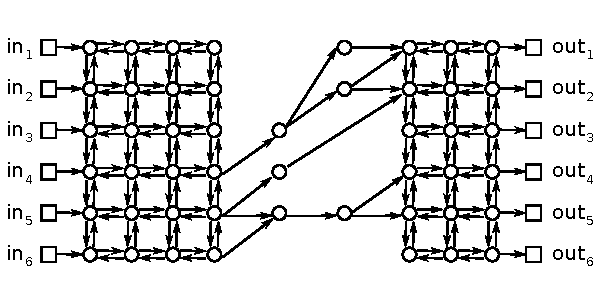
\includegraphics[scale=1.5]{ps5-figs/7.pdf}
            \caption{Grid, Interrupted.}
            \label{gridint}
        \end{center}
    \end{figure}

    \solution{
        The diameter is 15: the most distant pair of vertices is $in_1$ and $out_6$, and the shortest path between them has length 15.
        
        The congestion is 2. This turns out to take a lot more work than intended (for example, a large brute-force search), and a solution is not included.

        For what it's worth, the following argument shows that congestion is at most 3. Given any routing problem on this network, we will construct a routing of congestion at most 3. Imagine dividing the network into two sub-networks with a common boundary: one is the left grid of 6 rows and 4 columns, and the other consists of everything else, together with the three nodes $n_1$, $n_2$, $n_3$ in the bottom half of the rightmost column of the left grid. The purpose of this division is to divide routing problems into problems through the two sub-networks.

        In the left sub-network, a $4 \times 6$ grid, we will construct a routing for any desired mapping of the inputs to the "interface nodes" $n_1$, $n_2$, and $n_3$, so long as that mapping only maps two inputs to each interface node. The routing is as follows. The routes from inputs $\mathsf{in}_4$, $\mathsf{in}_5$, and $\mathsf{in}_6$ traverse the first column until they reach the row of the correct interface node, and then they travel horizontally. The other three routes move right until they reach a particular column: the second column for $\mathsf{in}_3$, the third column for $\mathsf{in}_2$, and the fourth column for $\mathsf{in}_1$; and then the routes travel down the grid to the appropriate row and travel right to the appropriate node. This routing on the left grid sub-network has congestion at most three.

        In the right sub-network, it is easy enough to draw a congestion 3 routing for the following specific problem: $n_1$ to $\mathsf{out}_1$ and $\mathsf{out}_2$, $n_2$ to $\mathsf{out}_3$ and $\mathsf{out}_4$, and $n_3$ to $\mathsf{out}_5$ and $\mathsf{out}_6$. (This isn't a permutation, so it's not technically a routing problem by the book, but the meaning should be clear. And in fact a congestion 2 routing exists for this part.)

        Now, given any routing problem for the full network (i.e.\ any bijection between inputs and outputs), we split it into two routing sub-problems as follows: any inputs destined for the first two outputs will route through $n_1$; any inputs destined for the third or fourth outputs will route through $n_2$; and the remaining two will route through $n_3$. The above constructions describe sub-network routings that we can combine to achieve this with congestion at most $3$.

        It's clear that the network doesn't have congestion $1$: the three nodes $n_1$, $n_2$, and $n_3$ are a bottleneck, forbidding a congestion $1$ routing for all routing problems on this network. So we have at least argued that the congestion is $2$ or $3$.

    }

\end{problem}







% P8
\begin{problem}{10}
    Construct a $16$-bit de Bruijn sequence, by considering an Eulerian tour of the de Bruijn graph.

    \solution{
        We find an Euler tour of the de Bruijn graph, and read off the labels as we traverse the tour: $0111100101000011$.
    }

\end{problem}

\end{document}
